\section{Fonctions de hachage en éponge}

\begin{frame}<handout:0>
  \frametitle{Plan}
  \tableofcontents[currentsection,subsectionstyle=hide]
\end{frame}

\begin{frame}
  \frametitle{Etat d'une fonction en éponge}
  \vfill
  \begin{itemize}
  \item $S$: l'état (state) de la fonction $S = R \vert \vert C$.
    \item $R$: partie externe de l'état, les premier $r$ bits de l'état.
  \item $C$: partie interne de l'état, de taille $c=b-r$ bits.
  \end{itemize}
 \begin{figure}[H]
        \centering
        \begin{tikzpicture}[scale=0.7]
    
        \draw [fill=red!70!grey, line width=2pt] (-0.5,-3) rectangle (0.5,-1);
        \draw [fill=green!80, line width=2pt] (-0.5,-1) rectangle (0.5,3);
        
        \node [align=center] at (0,1){\textbf{$R$}};
        \node [align=center]   at (0,-2){\textbf{$C$}};

        \node [align=center] at (-1.3,1){\textbf{$r$}};        
        \node [align=center] at (-2.2,-2){\textbf{$c =b-r$}};        

        \node [align=center] at (1.4,0){\textbf{$b$}}; 
        
        \draw [<->, >=latex, line width=1pt, color=red!70!grey] (-1,-3) -- (-1,-1);
        \draw [<->, >=latex, line width=1pt, color=green!80] (-1,-1) -- (-1,3);
        \draw [<->, >=latex, line width=1pt, color=grey] (1,-3) -- (1,3);
    
        \end{tikzpicture}
    \caption{État d'une fonction en éponge.}
    \end{figure}
  \vfill
\end{frame}

\begin{frame}
  \frametitle{Construction en éponge}
  \vfill
\begin{figure}[H]
\centering
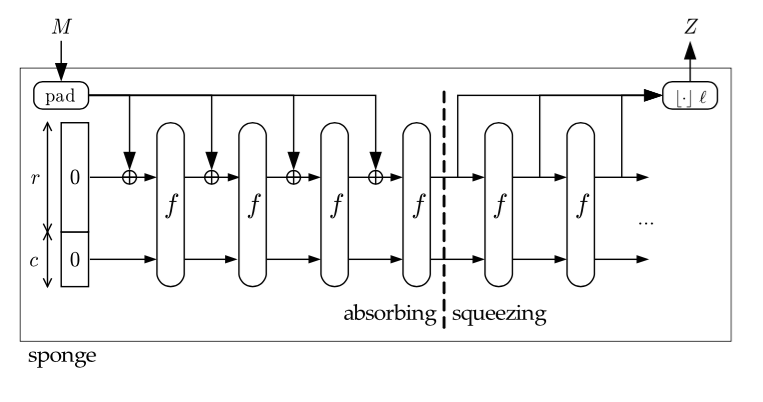
\includegraphics[scale=0.4]{sponge1.png}
\caption{Construction de fonctions en éponge $Z = \textsc{sponge}\lbrack f , pad, r\rbrack (M, l)$}
\end{figure}
  \vfill
\end{frame}

\begin{frame}
  \frametitle{Keccak formellement}
  \vfill
  
    \textbf{Paramètres de la fonction \textsc{Keccak}$\lbrack b, n_r \rbrack$ }:\\
  \begin{itemize}
  \item{ \textbf{$w$}: la longueur fixée des chaines de bits permutés.
  
  \hspace{1cm}$w=2^l$ bits, avec $0 \le l \le 6$.
  }
  \item{ \textbf{$n_r$}: le nombre d'itérations effectuées des routines internes.
  
  \hspace{1cm}$n_r = 12+2\times l$.
  }
  \end{itemize}
  \vspace{1cm}
  \textbf{État de la fonction \textsc{Keccak}}
\begin{itemize}
\item{État constitué de $b = 5 \times 5 \times w$ bits.}
\item{État représenté sous forme matricielle:
\begin{itemize}
\item $5\times w$ lignes indexées horizontalement par x, $0 \le x < 5$.
\item $5 \times w$ colonnes indexées verticalement par y, $0 \le y < 5$.
\item $25$ mots (ou rangées) indexées en profondeur par z, $0 \le z < w$.
\end{itemize}
}
\item{$A\lbrack x,y,z\rbrack$ permet d'accéder à tous les bits de l'état.}
\end{itemize}

  \vfill
\end{frame}

\begin{frame}[fragile]
  \frametitle{État de la fonction Keccak:\\ Représentation matricielle}
  \vfill
  \begin{figure}[H]
    \centering
    \begin{tikzpicture}[scale=0.3]

      \newcommand\faceside[6]{
        \draw (-2+#4,-1+#5) node[]{} node{$\bullet$};
        \pgfmathparse{#1/2+#4}
        \node[text centered, font=\bf] at (\pgfmathresult,-0.7+#5) {#6};
        \foreach \a in {1,...,#1} {
          \foreach \b in {1,...,#2} {
            \fill[fill=white, draw=black] (#4+-1+\a,#5+-1+\b) -- (#4+\a,#5+-1+\b) -- (#4+\a,#5+\b) -- (#4+-1+\a,#5+\b) -- cycle;
          }
          \pgfmathparse{-1+#3}
          \foreach \d [evaluate=\d as \dd using \d*0.5] in {0,...,\pgfmathresult} {
            \fill[fill=white, draw=black] (#4+-1+\a+\d-\dd,#5+#2+\d-\dd) -- (#4+\a+\d-\dd,#5+#2+\d-\dd) -- (#4+\a+\d+0.5-\dd,#5+#2+\d+0.5-\dd) -- (#4+\a+\d-0.5-\dd,#5+#2+\d+0.5-\dd) -- cycle;
          }
        }
        \foreach \c in {1,...,#2} {
          \pgfmathparse{-1+#3}
          \foreach \e [evaluate=\e as \ee using \e*0.5] in {0,...,\pgfmathresult} {
            \fill[fill=white, draw=black] (#4+#1+\e-\ee,#5+-1+\c+\e-\ee) -- (#4+#1+\e+0.5-\ee,#5+-1+\c+\e+0.5-\ee) -- (#4+#1+\e+0.5-\ee,#5+0.5+\c+\e-\ee) -- (#4+#1+\e-\ee,#5+\c+\e-\ee) -- cycle;
          }
        }
      }

      \faceside{1}{1}{1}{-10}{11}{bit}
      \faceside{5}{1}{1}{0}{11}{row}\draw [->, >=latex, dashed] (-2,10) -- (-1,10);\draw (-0.6,10) node[]{$x$};
      \faceside{1}{5}{1}{10}{11}{column}\draw [->, >=latex, dashed] (8,10) -- (8,11);\draw (8,11.4) node[]{$y$};
      \faceside{1}{1}{2}{20}{11}{lane}\draw [->, >=latex, dashed] (18,10) -- (18.8,10.8);\draw (19.1,11.2) node[]{$z$};
      \faceside{5}{1}{2}{-10}{0}{plane}\draw [->, >=latex, dashed] (-12,-1) -- (-11,-1);\draw [->, >=latex, dashed] (-12,-1) -- (-11.1,-0.2);\draw (-10.6,-1) node[]{$x$};\draw (-10.9,0.2) node[]{$z$};
      \faceside{5}{5}{1}{0}{0}{slice}\draw [->, >=latex, dashed] (-2,-1) -- (-1,-1);\draw [->, >=latex, dashed] (-2,-1) -- (-2,0);\draw (-0.6,-1) node[]{$x$};\draw (-2,0.4) node[]{$y$};
      \faceside{1}{5}{2}{10}{0}{sheet}\draw [->, >=latex, dashed] (8,-1) -- (8,0);\draw [->, >=latex, dashed] (8,-1) -- (8.8,-0.2);\draw (8,0.4) node[]{$y$};\draw (9.1,0.2) node[]{$z$};
      \faceside{5}{5}{2}{20}{0}{state}\draw [->, >=latex, dashed] (18,-1) -- (19,-1);\draw [->, >=latex, dashed] (18,-1) -- (18,0);\draw [->, >=latex, dashed] (18,-1) -- (18.8,-0.2);\draw (19.4,-1) node[]{$x$};\draw (18,0.4) node[]{$y$};\draw (19.1,0.2) node[]{$z$};
      
    
    \end{tikzpicture}
    %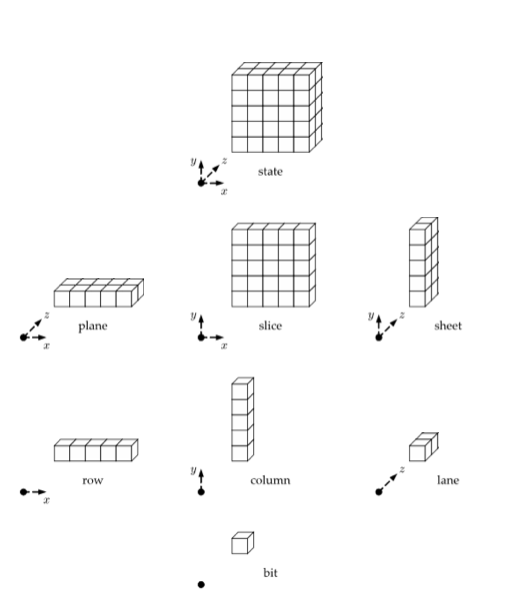
\includegraphics[scale=0.3]{StateArray.png}
    \caption{État manipulé sous forme matricielle A avec $x,y,z \in\llbracket 0,5 \llbracket \times \llbracket 0,5 \llbracket \times \llbracket 0,w \llbracket$}
  \end{figure}
  \vfill
\end{frame}

\begin{frame}
  \frametitle{Une Ronde de \textsc{Keccak}: \textsc{Rnd}}
  \vfill
  \textsc{Keccak}: Pour i de 1 à 24 faire: 
$$\textsc{Rnd}(A,i_r)=\iota ( \chi ( \pi ( \rho (\Theta (A)))), i_r)$$
\vspace{1cm}
Les routines d'une ronde \textbf{Rnd}:
  \begin{itemize}
  \item{La routine $\Theta$}
  \item{La routine $\rho$}
  \item{La routine $\pi$}
  \item{La routine $\chi$}
  \item{La routine $\iota$}
   \end{itemize}
  \vfill
\end{frame}

\begin{frame}
  \frametitle{SHA-3: Généralités}
  \vfill
\begin{itemize}
\item{\textbf{2 novembre 2007:} Publication par le National Institute of         Standards and Technology (NIST) annonçant la recherche d'algorithmes candidats pour une nouvelle famille de fonctions de hachage cryptographiques: SHA-3}
  \vfill
        \item{
        \textbf{Exigences générales}:
                \begin{itemize}
                \item{Condensés de 224, 256, 384, 512 bits }
                \item{Fournir une alternative à SHA-2 (bien que SHA-2 soit encore                 utilisable).}
                \item{Processus similaire à la compétition AES}
                \end{itemize}
        }
\end{itemize}
\vfill
\end{frame}

\begin{frame}
\vfill
   
\centerline{\textbf{SHA-3 implémente \textsc{Keccak}$\lbrack 1600, 24 \rbrack$}}
 
\bgroup
\def\arraystretch{1.5}
  \begin{table}
\begin{tabular}{l | c | c | c }
$w$ & $l$ & $n_r$ & $b$ \\
\hline
$2^6$ & $6$ & $24$ & $1600 $ 
\end{tabular}
\caption{Paramètres de la fonction \textsc{Keccak} pour SHA-3}

\end{table}

\egroup

\vfill

\textbf{Taille des condensés:}
\begin{itemize}
\item{Fonctions de hachage: 224, 256, 384 et 512 bits}
\item{Fonctions à sortie de taille variable: \textsc{SHAKE128}$(M,l)$ et \textsc{SHAKE128}$(M,l)$  pour une capacité de 256 bits, et une sortie de longueur $l$ }
\end{itemize}
\vspace{1cm}
\vfill
\end{frame}
